\documentclass[floatfix,aps,pra,twocolumn,superscriptaddress,10pt,nofootinbib]{revtex4-2}

\usepackage{graphicx}
\usepackage{bm}
\usepackage{booktabs}
\usepackage[title]{appendix}
\usepackage{float}
\usepackage{ragged2e}
\usepackage{amsmath,amssymb}
\usepackage{xcolor}
\usepackage{tikz}
\usetikzlibrary{arrows.meta,positioning,calc,decorations.pathreplacing,fit,backgrounds}
\usepackage{hyperref}

% ---------------------------------------------------------------------
% Colours used consistently in every figure (quantum/QPU = orange, classical = blue, FakeBerlin = aqua)
\definecolor{qcol}{HTML}{EB6834}
\definecolor{ccol}{HTML}{2A78D6}
\definecolor{fcol}{HTML}{1BAF7A}

% Working notes -- set \showtodostrue -> \showtodosfalse to hide them all
\newif\ifshowtodos \showtodostrue
\newcommand{\TODO}[1]{\ifshowtodos\textcolor{red}{\textbf{[TODO:} #1\textbf{]}}\fi}

\newtheorem{proposition}{Proposition}
\newtheorem{remark}{Remark}
\newcommand{\sg}{\operatorname{sg}}
\newcommand{\Ncol}{N_{\rm col}}

% Algorithms without extra packages: numbered, ruled, non-floating blocks
% (revtex4-2 and the float package's \newfloat do not combine)
\newcounter{algorithm}
\newenvironment{algorithm}[1]{\par\medskip\noindent\begin{minipage}{\linewidth}\refstepcounter{algorithm}%
  \hrule height 0.6pt\vspace{2pt}\noindent{\small\textbf{Algorithm~\thealgorithm.} #1}\vspace{2pt}\hrule height 0.3pt%
  \small\begin{list}{\arabic{enumi}:}{\usecounter{enumi}\setlength{\itemsep}{1pt}%
  \setlength{\parsep}{0pt}\setlength{\topsep}{3pt}\setlength{\leftmargin}{1.5em}\setlength{\labelwidth}{1.2em}}}%
  {\end{list}\vspace{2pt}\hrule height 0.6pt\end{minipage}\par\medskip}

\hypersetup{colorlinks=true, linkcolor=blue!50!black, citecolor=blue!50!black, urlcolor=blue!50!black}

\graphicspath{{figures/}}

\begin{document}

\title{Training a physics-informed neural network with a fixed quantum layer on a superconducting quantum processor}
% Alternative titles:
%  - "Hybrid quantum physics-informed neural networks trained with the quantum processor in the loop"
%  - "A non-variational quantum layer for physics-informed learning, from noiseless simulation to 80 superconducting qubits"

\author{Gubio G. de Lima}
\email{gubio.gomes@estudante.ufscar.br}
\affiliation{\TODO{afilia\c{c}\~ao (CBPF / UFSCar)}}

\author{Erick \TODO{sobrenome}}
\affiliation{\TODO{afilia\c{c}\~ao}}

\begin{abstract}
\TODO{Resumo -- a escrever por \'ultimo.}
\end{abstract}

\maketitle

% =====================================================================
\section{Introduction}\label{sec:intro}
% =====================================================================
\TODO{Introdu\c{c}\~ao -- a escrever.}
% Suggested storyline (structure modelled on Refs. [havlicek2019supervised, wright2022deep, kyriienko2021solving]):
%  1. PINNs [raissi2019physics, karniadakis2021physics] and their training pathologies at small collocation
%     budgets and long horizons [krishnapriyan2021characterizing, wang2021understanding, wang2022when].
%  2. Quantum circuits for differential equations [lubasch2020variational, kyriienko2021solving, paine2023quantum]
%     and hybrid quantum PINNs [sedykh2024hybrid, berger2025trainable, farea2025qcpinn, lantigua2026classical,
%     zabihi2026hybrid]: trainable (variational) circuits, noiseless simulation, barren plateaus
%     [mcclean2018barren, cerezo2021cost], gradients by parameter shift [mitarai2018quantum, schuld2019evaluating].
%  3. Fixed (non-variational) quantum feature maps exist [havlicek2019supervised, fujii2017harnessing,
%     mujal2021opportunities, henderson2020quanvolutional] but not inside a physics-informed residual.
%  4. Gap: no PINN has been TRAINED on a quantum processor; the FD residual amplifies shot noise.
%  5. This work: fixed quantum layer + calibrated trigonometric surrogate + straight-through gradient
%     (physics-aware training [wright2022deep]); same-protocol comparison in simulation (2800 runs per model);
%     training with 80 qubits of ibm_berlin in the loop (1 job per epoch); honest framing with respect to
%     classical surrogates [schreiber2023classical].
%  6. Outline.

% =====================================================================
\section{Theoretical framework}\label{sec:theory}
% =====================================================================

\subsection{Benchmark problem}\label{sec:problem}
We solve the viscous Burgers equation on the periodic unit interval,
\begin{equation}
  \partial_t u + u\,\partial_x u = \nu\,\partial_x^2 u,\qquad x\in[0,1),\ t\in[0,T],
  \label{eq:burgers}
\end{equation}
with $u(x+1,t)=u(x,t)$, $u(x,0)=\sin(2\pi x)$ and $\nu=0.01$. Equation~\eqref{eq:burgers} is the simplest partial differential equation (PDE) that combines nonlinear advection with diffusion~\cite{basdevant1986spectral}: for $\nu=0.01$ the initial sine steepens into a front at $x=1/2$, which is already sharp at $T=0.1$; at $T=1$ the wave has been strongly damped ($\|u\|_{\rm rms}\simeq0.21$) and the problem is harder for the networks because the solution has to be propagated over a ten times longer horizon. We consider the \emph{forward} problem: $\nu$ is known and no solution data enter the training. A reference solution $u_{\rm FDM}$ is computed by explicit finite differences (Appendix~\ref{app:reference}) and is used only for evaluation. The accuracy of a model is measured on $u(x,T)$ at 200 equispaced points by the mean squared error (MSE) and the relative $L_2$ error $\epsilon_{L_2}=\|u-u_{\rm FDM}\|_2/\|u_{\rm FDM}\|_2$. A model that does not evolve the initial condition, $u(x,T)=\sin2\pi x$, has $\mathrm{MSE}=3.93\times10^{-2}$ at $T=0.1$ and $2.82\times10^{-1}$ at $T=1$; we refer to this as the \emph{no-evolution level}.

\subsection{Physics-informed neural networks}\label{sec:pinn}
A physics-informed neural network (PINN)~\cite{raissi2019physics,karniadakis2021physics} represents the solution by a parametrized function $u_\Theta(x,t)$ and determines the parameters $\Theta$ by minimizing the residual of the PDE at a set of collocation points $\{(x_i,t_i)\}_{i=1}^{\Ncol}$,
\begin{equation}
  \mathcal L(\Theta)=\frac{1}{\Ncol}\sum_{i=1}^{\Ncol} r_i^2,
  \label{eq:loss}
\end{equation}
with $r_i=\big(\partial_t u_\Theta+u_\Theta\,\partial_x u_\Theta-\nu\,\partial_x^2u_\Theta\big)(x_i,t_i)$.
Boundary and initial conditions are usually added as penalty terms; here both are imposed exactly by construction~\cite{lagaris1998artificial}. The network acts on the periodic feature vector $\bm\xi(x,t)=(\sin2\pi x,\cos2\pi x,t/T)$ and its output enters
\begin{equation}
  u_\Theta(x,t)=\sin(2\pi x)+\frac{t}{T}\,\big(\mathcal N_{\rm post}\circ\mathcal M\circ\mathcal N_{\rm pre}\big)\big(\bm\xi(x,t)\big),
  \label{eq:composition}
\end{equation}
so that $u_\Theta$ is exactly 1-periodic in $x$ and equals the initial condition at $t=0$, and Eq.~\eqref{eq:loss} is the complete loss. The classical pre-network $\mathcal N_{\rm pre}(\cdot;\bm\phi):\mathbb R^3\to\mathbb R^n$ (one hidden layer of 10 $\tanh$ units, linear output) maps the features to a latent vector $\bm\theta\in\mathbb R^n$, a middle block $\mathcal M:\mathbb R^n\to\mathbb R^n$ transforms it into $\bm y$, and the classical post-network $\mathcal N_{\rm post}(\cdot;\bm\psi):\mathbb R^n\to\mathbb R$ (one hidden layer of 10 $\tanh$ units) produces the correction to the initial profile [Fig.~\ref{fig:schematic}(a)]. The width $n$ of the latent space is the only size parameter of the model. The classical PINN and the hybrid quantum PINN (HQPINN) differ \emph{only} in $\mathcal M$, so that any difference in their behaviour can be attributed to the middle block.

The derivatives in $r_i$ are computed by second-order central differences of the network itself on the five-point stencil $\{(x_i,t_i),(x_i\pm h,t_i),(x_i,t_i\pm\tau)\}$ with $h=1/512$ and $\tau=10^{-3}$ [Fig.~\ref{fig:schematic}(b)], rather than by automatic differentiation with respect to the inputs. This choice is dictated by the hardware: a quantum processor returns function values, not derivatives with respect to $(x,t)$, and all stencil nodes of a batch can be evaluated in a single pass. The truncation error of the stencil is negligible at the accuracy reached here (Appendix~\ref{app:ste}). At every optimizer step a fresh set of $\Ncol$ collocation points is drawn uniformly in $[0,1)\times[\tau,T-\tau]$.

In the \emph{classical PINN} the middle block is a trainable network,
\begin{equation}
  \mathcal M_{\rm C}(\bm\theta)=\mathcal N_{\rm mid}(\bm\theta;\bm\chi),
  \label{eq:bottleneck}
\end{equation}
with one hidden $\tanh$ layer, so that the classical model is a $\tanh$ network $3\to10\to n\to m\to n\to10\to1$ with a bottleneck of width $n$; the hidden width is $m=n$ in the long-budget simulations and $m=10$ in the hardware-budget control (Table~\ref{tab:arch}; the two coincide at $n=10$, 491 parameters).

\subsection{Hybrid quantum PINN with a fixed quantum layer}\label{sec:hqpinn}
In the HQPINN the latent vector is the set of rotation angles of an $n$-qubit circuit,
\begin{equation}
  U(\bm\theta)=W_{\rm brick}\,\bigotimes_{q=1}^{n}R_Y(\theta_q),\qquad R_Y(\theta)=e^{-i\theta Y/2},
  \label{eq:circuit}
\end{equation}
where $W_{\rm brick}$ is one brickwork layer of nearest-neighbour CNOT gates, first on the pairs $(1,2),(3,4),\dots$ and then on $(2,3),(4,5),\dots$ ($n-1$ gates in total). The circuit acts on $|0\rangle^{\otimes n}$ and the layer output is the vector of local magnetizations,
\begin{equation}
  y_q(\bm\theta)=\operatorname{Tr}\!\big[Z_q\,\mathcal E_{\bm\theta}\big(|0\rangle\langle0|^{\otimes n}\big)\big],\qquad q=1,\dots,n,
  \label{eq:expval}
\end{equation}
where $\mathcal E_{\bm\theta}$ is the channel actually implemented by the device. On hardware $y_q$ is estimated from $S$ shots, $\hat y_q=y_q+\xi_q$ with $\mathbb E[\xi_q]=0$ and $\operatorname{Var}[\xi_q]=(1-y_q^2)/S\le1/S$.

The defining feature of the model is that \emph{the circuit has no free parameter}: all trainable parameters belong to the classical networks, and the quantum layer is a fixed nonlinear map $\bm\theta\mapsto\bm y$. The HQPINN has $21n+61$ trainable parameters (271 for $n=10$), roughly half of the classical model of the same width. This is the opposite design choice to the variational hybrid PINNs studied so far~\cite{sedykh2024hybrid,berger2025trainable,farea2025qcpinn,lantigua2026classical,zabihi2026hybrid}, and connects the HQPINN to fixed-substrate approaches such as quantum feature maps~\cite{havlicek2019supervised}, quantum reservoir computing and extreme learning machines~\cite{fujii2017harnessing,mujal2021opportunities} and quanvolutional networks~\cite{henderson2020quanvolutional}, none of which has been used to minimize a PDE residual.

\paragraph{Function class.} The structure of the quantum layer is captured by the following statement (proof in Appendix~\ref{app:trig}).
\begin{proposition}\label{prop:trig}
Let $\mathcal C_q\subseteq\{1,\dots,n\}$ be the backward light cone of $Z_q$ in the circuit~\eqref{eq:circuit}. For any noise model in which every gate is followed by a $\bm\theta$-independent, trace-preserving channel acting on the qubits of that gate (readout errors included), $y_q$ depends only on $\{\theta_j\}_{j\in\mathcal C_q}$ and is a multilinear trigonometric polynomial of degree one in each of them,
\begin{equation}
  y_q(\bm\theta)=\sum_{\bm\alpha\in\{0,c,s\}^{|\mathcal C_q|}}c^{(q)}_{\bm\alpha}\prod_{j\in\mathcal C_q}g_{\alpha_j}(\theta_j),
  \label{eq:trigpoly}
\end{equation}
with $g_0=1$, $g_c=\cos$, $g_s=\sin$, and device-dependent real coefficients $c^{(q)}_{\bm\alpha}$. For one brickwork layer $|\mathcal C_q|\le4$, i.e., at most $3^4=81$ coefficients per output.
\end{proposition}
The hypothesis holds on IBM devices because $R_Y(\theta)$ is compiled into fixed microwave pulses and a \emph{virtual} $R_Z$ rotation, so the physical operations, and hence their errors, do not depend on $\theta$. Equation~\eqref{eq:trigpoly} has three consequences that guide both the theory and the implementation. (i) The quantum layer injects a finite Fourier structure into the latent representation~\cite{schuld2021effect}: the pre-network learns where to place the angles, and the circuit multiplies harmonics of different latent coordinates, $\cos\theta_a\cos\theta_b=\tfrac12[\cos(\theta_a+\theta_b)+\cos(\theta_a-\theta_b)]$, in the spirit of Fourier-feature networks~\cite{tancik2020fourier,rahimi2007random}. (ii) Noise does not change the function class, only the coefficients; this is what makes a calibrated surrogate of the device possible (Sec.~\ref{sec:hil}). (iii) The quantum layer has no trainable parameter, so the barren-plateau phenomenon of variational circuits~\cite{mcclean2018barren,cerezo2021cost} does not arise; what remains is the possible concentration of the map $\bm\theta\mapsto\bm y$ itself, which is controlled by the size of the light cones (Remark~\ref{rem:parity}).

\begin{remark}\label{rem:parity}
A CNOT network acts on the computational basis as a linear map over $\mathrm{GF}(2)$, $\bm b\mapsto M\bm b$. For the noiseless circuit~\eqref{eq:circuit} the Heisenberg evolution of $Z_q$ is the Pauli string $\prod_{j\in\mathcal S_q}Z_j$ with $\mathcal S_q=\{j:M_{qj}=1\}\subseteq\mathcal C_q$, and
\begin{equation}
  y_q(\bm\theta)=\prod_{j\in\mathcal S_q}\cos\theta_j ,\qquad |\mathcal S_q|\le3 .
  \label{eq:parity}
\end{equation}
The ideal layer is therefore efficiently classically computable: the noiseless HQPINN is a classical network with cosine-product activations. Its simulation results (Sec.~\ref{sec:res_sim}) measure the merit of this \emph{architecture}, not a quantum advantage, in line with the general results on classical surrogates of quantum learning models~\cite{schreiber2023classical}. For angles spread over a full period, $\operatorname{Var}[y_q]=2^{-|\mathcal S_q|}$, so deeper entangling layers trade expressivity (longer products) against concentration.
\end{remark}

\subsection{Training with the quantum processor in the loop}\label{sec:hil}
Training the HQPINN on a quantum processor raises two problems. First, the device returns $\hat{\bm y}$ but not $\partial\bm y/\partial\bm\theta$. Parameter-shift rules~\cite{mitarai2018quantum,schuld2019evaluating,wierichs2022general} give unbiased derivatives at the price of $2n$ extra circuits per evaluation point, and SPSA~\cite{spall1992multivariate,kandala2017hardware} gives a single random directional derivative per step. Second, the residual~\eqref{eq:loss} is built from finite differences: if the five stencil nodes were measured independently, the shot noise $\sigma_u$ of $u$ would enter $\partial_x^2u$ amplified by $\sqrt6/h^2\approx6.4\times10^5$ (Appendix~\ref{app:ste}), which would bury the physical signal. Both problems are solved by Proposition~\ref{prop:trig}, through a scheme analogous to the physics-aware training of physical neural networks~\cite{wright2022deep}, in which the physical system computes the forward pass and a digital model of it provides the backward pass [Fig.~\ref{fig:schematic}(c)]:
\begin{enumerate}
  \item \emph{Calibration.} Before training, one job evaluates the circuit at random angles $\theta_j\sim\mathcal U(-\pi,\pi)$ on every $n$-qubit chain of the chip in parallel. The coefficients of Eq.~\eqref{eq:trigpoly} are obtained by linear least squares, which yields a classical surrogate $\hat f(\bm\theta)$ of the device with its average noise built in~\cite{sung2020using}.
  \item \emph{Training.} At each epoch the device is measured only at the $\Ncol$ stencil centres $\bm\theta_c$. Every node $\bm\theta$ of the stencil centred at $c$ receives
  \begin{equation}
    \tilde{\bm y}(\bm\theta)=\hat f(\bm\theta)+\sg\!\big[\hat{\bm y}^{\,\rm QPU}(\bm\theta_c)-\hat f(\bm\theta_c)\big],
    \label{eq:ste}
  \end{equation}
  where $\sg$ stops the gradient (straight-through estimator~\cite{bengio2013estimating}). At the centre $\tilde{\bm y}=\hat{\bm y}^{\,\rm QPU}$, so the value of $u$ entering the nonlinear term $u\,\partial_xu$ is the measured one; across the stencil the variation of $\tilde{\bm y}$ is that of the smooth surrogate, so the shot noise is not amplified by the finite differences; and the gradient is $\partial\tilde{\bm y}/\partial\bm\theta=\partial\hat f/\partial\bm\theta$, available analytically. Every $K_{\rm fit}$ epochs the surrogate is refitted with the calibration data and all measurements accumulated so far, so that it tracks the device in the region of angles actually visited by the network.
  \item \emph{Validation.} A final job evaluates $u(x,T)$ with the trained network and the circuit run on the device.
\end{enumerate}
A training run of $K$ epochs therefore costs $K+2$ jobs and $\Ncol$ circuit evaluations per epoch, independently of the number of trainable parameters (Table~\ref{tab:cost}). Because the surrogate has the exact functional form of the device response, the method does not approximate the circuit; its only bias is the statistical error of the fitted coefficients and the part of the device behaviour that the time-independent, chip-averaged model~\eqref{eq:trigpoly} cannot capture (chain-to-chain variation, drift, crosstalk), which we quantify in Sec.~\ref{sec:res_device}.

\begin{figure*}[t]
  \centering
  \resizebox{\textwidth}{!}{% Fig. 1 -- classical PINN and hybrid quantum PINN (HQPINN): architecture and training workflow.
% \input inside a figure* (main.tex wraps it in \resizebox{\textwidth}{!}{...}).
% Needs the TikZ libraries arrows.meta, positioning, calc, decorations.pathreplacing, the package bm,
% and the colours qcol (HQPINN / QPU) and ccol (classical) defined in main.tex.
% Preview alone: see run/paper_tools/schematic_preview.tex
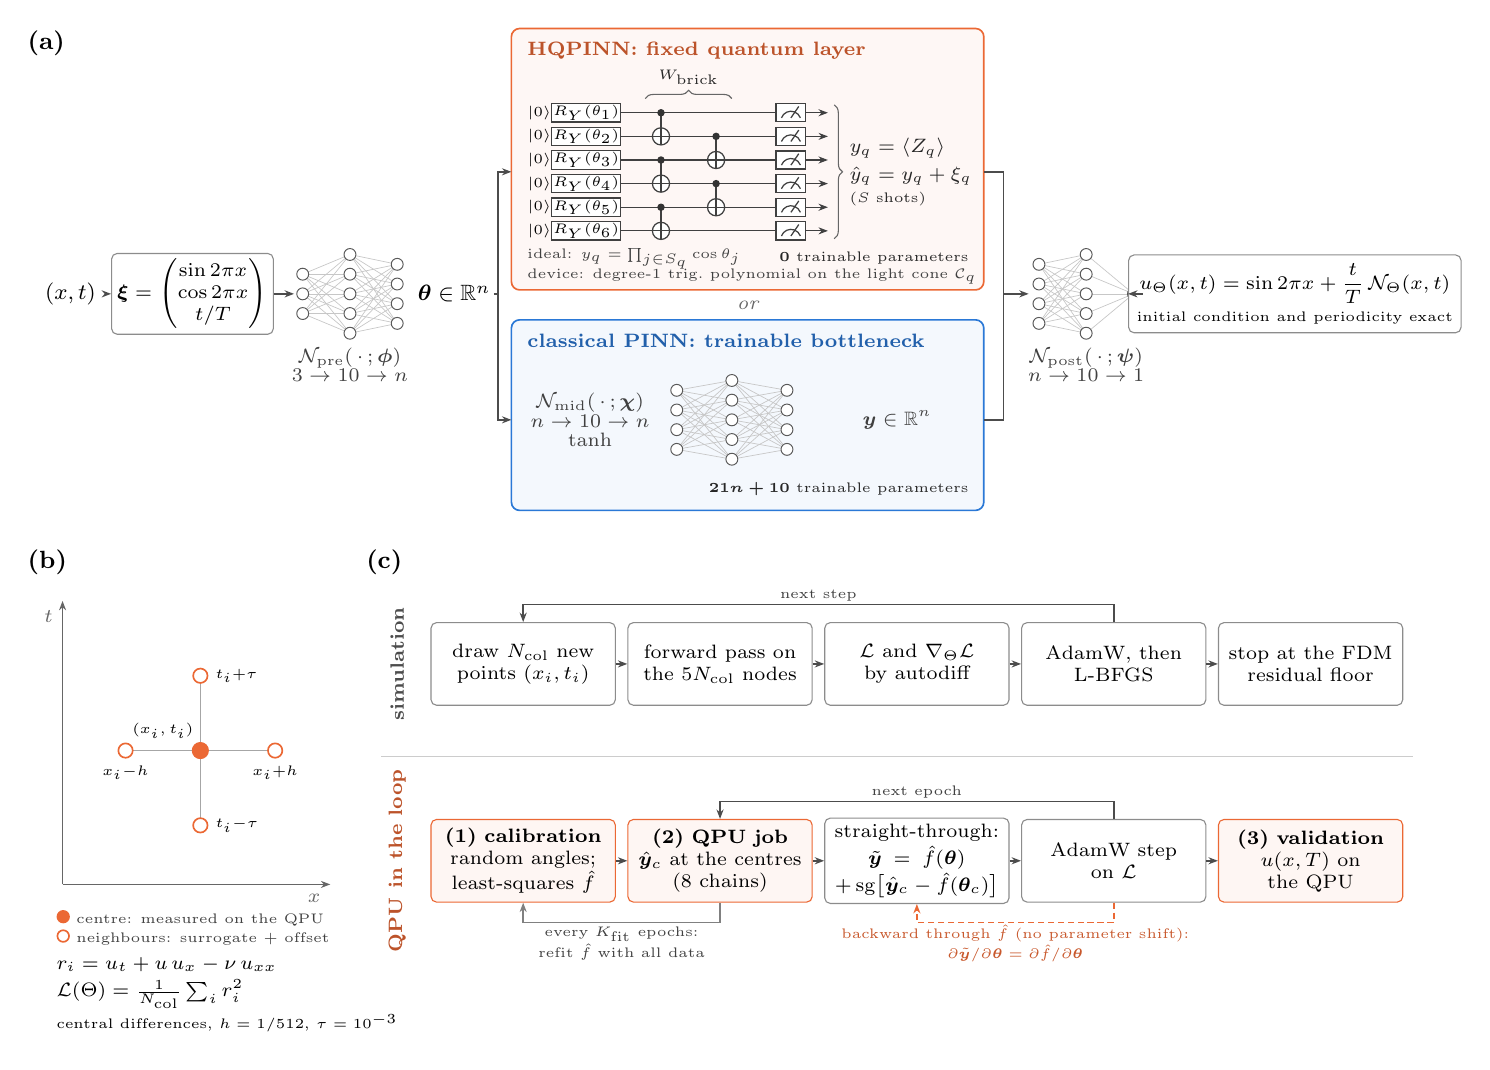
\begin{tikzpicture}[
  font=\footnotesize, >={Stealth[length=3.4pt]},
  arr/.style={->, line width=0.55pt, black!70},
  grad/.style={->, line width=0.6pt, qcol, dash pattern=on 2.2pt off 1.4pt},
  box/.style={draw=black!45, rounded corners=2pt, fill=white, align=center, font=\scriptsize,
              inner sep=2pt, text width=2.2cm, minimum height=1.05cm},
  qbox/.style={box, draw=qcol, fill=qcol!6},
  neuron/.style={circle, draw=black!65, fill=white, line width=0.35pt, inner sep=0pt, minimum size=4.3pt},
  wire/.style={black!75, line width=0.45pt},
  gate/.style={draw=black!75, fill=white, line width=0.45pt, inner sep=0.6pt, minimum height=0.23cm,
               minimum width=0.66cm, font=\tiny},
  plabel/.style={font=\small\bfseries, anchor=north west, inner sep=0pt},
  note/.style={font=\scriptsize, black!75, align=center},
  tnote/.style={font=\tiny, black!75},
]
% ---- helpers: a column of neurons, all-to-all links between two columns, CNOT, meter
\def\ncol#1#2#3{\foreach \i in {1,...,#2}{\node[neuron] at (#1,{#3+(\i-(#2+1)/2)*0.25}) {};}}
\def\nlinks#1#2#3#4#5{\foreach \i in {1,...,#2}{\foreach \j in {1,...,#4}{%
  \draw[black!22, line width=0.25pt] (#1,{#5+(\i-(#2+1)/2)*0.25}) -- (#3,{#5+(\j-(#4+1)/2)*0.25});}}}
\def\cnot#1#2#3{\draw[wire] (#1,#2) -- (#1,#3); \fill[black!80] (#1,#2) circle (1.35pt);
  \draw[wire, fill=white] (#1,#3) circle (3.1pt);
  \draw[wire] ({#1-0.109},#3) -- ({#1+0.109},#3); \draw[wire] (#1,{#3-0.109}) -- (#1,{#3+0.109});}
\def\meter#1#2{\draw[wire, fill=white] ({#1-0.19},{#2-0.115}) rectangle ({#1+0.19},{#2+0.115});
  \draw[wire] ({#1-0.12},{#2-0.065}) arc (160:20:0.128); \draw[wire] (#1,{#2-0.065}) -- ({#1+0.1},{#2+0.08});}

% =====================================================================================
% (a) architecture: shared classical pre/post networks, interchangeable middle block
% =====================================================================================
\node[plabel] at (-0.1,6.1) {(a)};
\node (in) at (0.45,2.75) {$(x,t)$};
\node[draw=black!45, rounded corners=2pt, fill=white, inner sep=2pt, font=\scriptsize, align=center] (xi) at (2.0,2.75)
  {$\bm\xi=\begin{pmatrix}\sin 2\pi x\\ \cos 2\pi x\\ t/T\end{pmatrix}$};
\draw[arr] (in) -- (xi);
% pre-network 3 -> 10 -> n
\nlinks{3.4}{3}{4.0}{5}{2.75}\nlinks{4.0}{5}{4.6}{4}{2.75}
\ncol{3.4}{3}{2.75}\ncol{4.0}{5}{2.75}\ncol{4.6}{4}{2.75}
\draw[arr] (xi.east) -- (3.29,2.75);
\node[note] at (4.0,1.85) {$\mathcal N_{\rm pre}(\,\cdot\,;\bm\phi)$\\[-1pt]$3\to10\to n$};
\node[anchor=west, inner sep=1pt] (theta) at (4.82,2.75) {$\bm\theta\in\mathbb R^{n}$};
\coordinate (split) at (5.88,2.75);
\draw[line width=0.55pt, black!70] (theta.east) -- (split);

% ---- middle block, option 1: fixed quantum circuit (HQPINN)
\draw[qcol, line width=0.6pt, rounded corners=3pt, fill=qcol!5] (6.05,2.8) rectangle (12.05,6.12);
\node[anchor=north west, font=\scriptsize\bfseries, text=qcol!80!black] at (6.13,6.07) {HQPINN: fixed quantum layer};
\foreach \q/\y in {1/5.05,2/4.75,3/4.45,4/4.15,5/3.85,6/3.55}{
  \node[font=\tiny, anchor=east, inner sep=1pt] at (6.6,\y) {$|0\rangle$};
  \draw[wire] (6.6,\y) -- (9.41,\y);
  \node[gate] at (7.0,\y) {$R_Y(\theta_{\q})$};
  \meter{9.6}{\y}
  \draw[wire, ->] (9.79,\y) -- (10.07,\y);
}
\cnot{7.95}{5.05}{4.75}\cnot{7.95}{4.45}{4.15}\cnot{7.95}{3.85}{3.55}
\cnot{8.65}{4.75}{4.45}\cnot{8.65}{4.15}{3.85}
\draw[decorate, decoration={brace, amplitude=3pt}, black!60] (7.75,5.23) -- (8.85,5.23)
  node[midway, above=1.5pt, font=\tiny, black!85] {$W_{\rm brick}$};
\draw[decorate, decoration={brace, amplitude=3pt}, black!60] (10.15,5.15) -- (10.15,3.45)
  node[midway, right=2pt, font=\scriptsize, black!85, align=left]
  {$y_q=\langle Z_q\rangle$\\[2pt]$\hat y_q=y_q+\xi_q$\\[0pt]{\tiny ($S$ shots)}};
\node[tnote, anchor=west] at (6.13,3.2) {ideal: $y_q=\prod_{j\in S_q}\cos\theta_j$};
\node[tnote, anchor=west] at (6.13,2.97) {device: degree-1 trig.\ polynomial on the light cone $\mathcal C_q$};
\node[font=\tiny, anchor=east, black!85] at (11.98,3.2) {\textbf{0} trainable parameters};

% ---- middle block, option 2: trainable bottleneck (classical PINN)
\draw[ccol, line width=0.6pt, rounded corners=3pt, fill=ccol!5] (6.05,0.0) rectangle (12.05,2.42);
\node[anchor=north west, font=\scriptsize\bfseries, text=ccol!80!black] at (6.13,2.37) {classical PINN: trainable bottleneck};
\nlinks{8.15}{4}{8.85}{5}{1.15}\nlinks{8.85}{5}{9.55}{4}{1.15}
\ncol{8.15}{4}{1.15}\ncol{8.85}{5}{1.15}\ncol{9.55}{4}{1.15}
\node[note] at (7.05,1.15) {$\mathcal N_{\rm mid}(\,\cdot\,;\bm\chi)$\\[-1pt]$n\to10\to n$\\[-1pt]$\tanh$};
\node[note] at (10.95,1.15) {$\bm y\in\mathbb R^{n}$};
\node[font=\tiny, anchor=south east, black!85] at (11.98,0.06) {$\bm{21n+10}$ trainable parameters};
\node[font=\scriptsize\itshape, black!60] at (9.05,2.61) {or};

% ---- routing theta -> middle block -> post-network
\draw[arr] (split) |- (6.05,4.3);
\draw[arr] (split) |- (6.05,1.15);
\draw[line width=0.55pt, black!70] (12.05,4.3) -- (12.3,4.3) -- (12.3,1.15) -- (12.05,1.15);
\draw[arr] (12.3,2.75) -- (12.62,2.75);
% post-network n -> 10 -> 1
\nlinks{12.75}{4}{13.35}{5}{2.75}\nlinks{13.35}{5}{13.95}{1}{2.75}
\ncol{12.75}{4}{2.75}\ncol{13.35}{5}{2.75}\ncol{13.95}{1}{2.75}
\node[note] at (13.35,1.85) {$\mathcal N_{\rm post}(\,\cdot\,;\bm\psi)$\\[-1pt]$n\to10\to1$};
\node[draw=black!45, rounded corners=2pt, fill=white, font=\scriptsize, align=center, inner sep=3pt] (u) at (16.0,2.75)
  {$u_\Theta(x,t)=\sin 2\pi x+\dfrac{t}{T}\,\mathcal N_\Theta(x,t)$\\[2pt]
   {\tiny initial condition and periodicity exact}};
\draw[arr] (14.07,2.75) -- (u.west);

% =====================================================================================
% (b) physics-informed residual on a five-point stencil
% =====================================================================================
\node[plabel] at (-0.1,-0.5) {(b)};
\draw[->, black!60, line width=0.45pt] (0.35,-4.75) -- (3.75,-4.75) node[below left=0pt, font=\scriptsize] {$x$};
\draw[->, black!60, line width=0.45pt] (0.35,-4.75) -- (0.35,-1.15) node[below left=0pt, font=\scriptsize] {$t$};
\draw[black!35, line width=0.4pt] (1.15,-3.05) -- (3.05,-3.05) (2.1,-4.0) -- (2.1,-2.1);
\foreach \p/\l/\a in {{(3.05,-3.05)}/{$x_i{+}h$}/below, {(1.15,-3.05)}/{$x_i{-}h$}/below,
                      {(2.1,-2.1)}/{$t_i{+}\tau$}/right, {(2.1,-4.0)}/{$t_i{-}\tau$}/right}{
  \draw[qcol, line width=0.6pt, fill=white] \p circle (2.6pt);
  \node[font=\tiny, \a=2pt] at \p {\l};}
\fill[qcol] (2.1,-3.05) circle (3.1pt);
\node[font=\tiny, above left=1pt and -1pt] at (2.1,-3.05) {$(x_i,t_i)$};
\node[tnote, align=left, anchor=west] at (0.15,-5.3)
  {\tikz\fill[qcol] (0,0) circle (2.4pt); centre: measured on the QPU\\[1pt]
   \tikz\draw[qcol, line width=0.6pt] (0,0) circle (2.1pt); neighbours: surrogate $+$ offset};
\node[font=\scriptsize, align=left, anchor=west] at (0.15,-6.15)
  {$r_i=u_t+u\,u_x-\nu\,u_{xx}$\\[2pt]$\mathcal L(\Theta)=\frac{1}{N_{\rm col}}\sum_i r_i^2$\\[1pt]
   {\tiny central differences, $h=1/512$, $\tau=10^{-3}$}};

% =====================================================================================
% (c) training workflows
% =====================================================================================
\node[plabel] at (4.2,-0.5) {(c)};
\node[rotate=90, font=\scriptsize\bfseries, black!70] at (4.6,-1.95) {simulation};
\node[rotate=90, font=\scriptsize\bfseries, text=qcol!80!black] at (4.6,-4.45) {QPU in the loop};
\draw[black!20, line width=0.4pt] (4.4,-3.13) -- (17.5,-3.13);

% lane 1: simulation (classical PINN and ideal HQPINN)
\node[box] (s1) at (6.2,-1.95) {draw $N_{\rm col}$ new\\points $(x_i,t_i)$};
\node[box] (s2) at (8.7,-1.95) {forward pass on\\the $5N_{\rm col}$ nodes};
\node[box] (s3) at (11.2,-1.95) {$\mathcal L$ and $\nabla_\Theta\mathcal L$\\by autodiff};
\node[box] (s4) at (13.7,-1.95) {AdamW, then\\L-BFGS};
\node[box] (s5) at (16.2,-1.95) {stop at the FDM\\residual floor};
\draw[arr] (s1) -- (s2); \draw[arr] (s2) -- (s3); \draw[arr] (s3) -- (s4); \draw[arr] (s4) -- (s5);
\draw[arr] (s4.north) -- ++(0,0.22) -| (s1.north);
\node[tnote, fill=white, inner sep=1pt] at (9.95,-1.08) {next step};

% lane 2: HQPINN with the QPU in the loop
\node[qbox] (q0) at (6.2,-4.45) {\textbf{(1) calibration}\\random angles;\\least-squares $\hat f$};
\node[qbox] (q1) at (8.7,-4.45) {\textbf{(2) QPU job}\\$\hat{\bm y}_c$ at the centres\\(8 chains)};
\node[box] (q2) at (11.2,-4.45) {straight-through:\\[1pt]$\tilde{\bm y}=\hat f(\bm\theta)$\\$+\,\mathrm{sg}\big[\hat{\bm y}_c-\hat f(\bm\theta_c)\big]$};
\node[box] (q3) at (13.7,-4.45) {AdamW step\\on $\mathcal L$};
\node[qbox] (q4) at (16.2,-4.45) {\textbf{(3) validation}\\$u(x,T)$ on the QPU};
\draw[arr] (q0) -- (q1); \draw[arr] (q1) -- (q2); \draw[arr] (q2) -- (q3); \draw[arr] (q3) -- (q4);
\draw[arr] (q3.north) -- ++(0,0.22) -| (q1.north);
\node[tnote, fill=white, inner sep=1pt] at (11.2,-3.58) {next epoch};
\draw[grad] (q3.south) -- ++(0,-0.25) -| (q2.south);
\node[tnote, text=qcol!85!black, align=center] at (12.45,-5.5)
  {backward through $\hat f$ (no parameter shift):\\$\partial\tilde{\bm y}/\partial\bm\theta=\partial\hat f/\partial\bm\theta$};
\draw[arr, black!50] (q1.south) -- ++(0,-0.25) -| (q0.south);
\node[tnote, align=center] at (7.45,-5.5) {every $K_{\rm fit}$ epochs:\\refit $\hat f$ with all data};
\end{tikzpicture}
}
  \caption{\justifying
  Classical PINN and hybrid quantum PINN (HQPINN).
  (a) Architecture. Both models share the classical pre-network $\mathcal N_{\rm pre}$, which maps the periodic features $\bm\xi$ to the latent vector $\bm\theta\in\mathbb R^n$, and the classical post-network $\mathcal N_{\rm post}$; the initial condition and the periodicity are imposed exactly by Eq.~\eqref{eq:composition}. In the HQPINN (orange) the middle block is a \emph{fixed} quantum circuit---one $R_Y(\theta_q)$ rotation per qubit followed by one brickwork layer of CNOTs---whose output is the vector of local expectation values $y_q=\langle Z_q\rangle$, estimated with $S$ shots; the circuit has no trainable parameter. Six of the $n=10$ qubits used on hardware are drawn. In the classical PINN (blue) the middle block is a trainable bottleneck $\mathcal N_{\rm mid}$.
  (b) Physics-informed residual. The derivatives in $r_i$ are central differences of the network on a five-point stencil; on hardware only the centre is measured, and the neighbours receive the surrogate value plus the same measured offset [Eq.~\eqref{eq:ste}].
  (c) Training workflows. In simulation the full stencil is evaluated exactly and the gradient is obtained by automatic differentiation. With the quantum processor in the loop, (1) one calibration job fits the trigonometric surrogate $\hat f$ of the device [Eq.~\eqref{eq:trigpoly}]; (2) at every epoch one job measures the circuit at the $\Ncol$ stencil centres on all chains in parallel, the forward pass uses the measured values and the backward pass goes through $\hat f$ (straight-through estimator, dashed); $\hat f$ is refitted every $K_{\rm fit}$ epochs with all measurements; (3) one final job evaluates the trained network on the device.}
  \label{fig:schematic}
\end{figure*}

% =====================================================================
\section{Methods}\label{sec:methods}
% =====================================================================
The numerical and experimental protocols are summarized here; Appendices~\ref{app:training}--\ref{app:hyper} contain the full algorithms, the implementation of the hardware loop and all hyperparameters. The results are organized in two groups: \emph{simulations} (noiseless circuits, shot noise only, and the noise model of the device) and \emph{real-QPU} executions.

\subsection{Simulations}\label{sec:methods_sim}
\paragraph{Long-budget, same-protocol sweep.} Both models are trained with the same algorithm and hyperparameters (Algorithm~\ref{alg:sim}): AdamW~\cite{loshchilov2019decoupled} with learning rate $10^{-3}$ reduced on plateaus, a fresh batch of $\Ncol$ collocation points at every step, up to $2\times10^4$ steps, followed by at most $10^3$ L-BFGS iterations~\cite{liu1989limited} on the last batch. The residual is monitored on a fixed validation set of $\Ncol$ random points, and training stops when it reaches the residual of the reference solution itself on the same points and with the same stencil: below this \emph{FDM floor} the network would be fitting the discretization error of the reference. The best monitored snapshot is returned. We sweep $n=2,\dots,15$, $\Ncol\in\{10,100\}$ and $T\in\{0.1,1\}$, with 50 seeds per configuration and model (5600 runs), seed $s$ fixing the initialization and the validation set. \TODO{arquivar no reposit\'orio o script que gerou a varredura (\texttt{Experiment1Modified}, protocolo \texttt{fixed\_validation\_v2}); a vers\'ao local de \texttt{run\_qubit\_sweep.py} monitora o lote de treino.} The ideal quantum layer is evaluated with the closed form~\eqref{eq:parity}, which is exact for the noiseless circuit and differentiable. A complementary sweep of the HQPINN alone covers $\Ncol$ from 10 to 500 for $n\in\{3,5,7,10,15\}$ (Appendix~\ref{app:extra}).

\paragraph{Hardware-budget simulations.} To separate the effect of noise from that of the short training affordable on hardware, the HQPINN is also trained offline with exactly the protocol of the hardware run (110 epochs, $\Ncol=10$, same learning-rate schedule, same initialization and collocation stream per seed; Sec.~\ref{sec:methods_hw}) with (i) the ideal layer on all stencil nodes and (ii) the ideal layer plus binomial shot noise with $S=1024$ at the stencil centres, propagated with Eq.~\eqref{eq:ste} and a perfect surrogate. Seeds 0--4 are used.

\paragraph{Noisy emulation.} The device is emulated with the \texttt{FakeBerlin} noise model of Qiskit~\cite{javadiabhari2024qiskit}, which reproduces the calibrated gate errors, $T_1/T_2$ relaxation, readout errors and coupling map of \texttt{ibm\_berlin} but not crosstalk or temporal drift. Each 10-qubit chain is simulated exactly as a density matrix and $S=1024$ shots are sampled. The emulated training uses the same physical chains, seed, collocation stream and protocol as the real run (Algorithm~\ref{alg:hil}).

\subsection{Real-QPU execution}\label{sec:methods_hw}
The hardware experiment ran on \texttt{ibm\_berlin}, an IBM Nighthawk processor with 120 transmon qubits on a square lattice and native CZ gates, on 8 October 2026, within a single dedicated runtime \texttt{Session}. The circuit~\eqref{eq:circuit} with $n=10$ was laid out on 8 disjoint chains of 10 coupled qubits [Fig.~\ref{fig:hardware}(a)], selected from the current calibration data (12 candidate chains, 4 discarded for a high error score), and the 8 copies were transpiled into a single packed circuit of depth 12 with 72 CZ gates and no SWAPs. All expectation values were estimated with $S=1024$ shots (precision $1/32$) and \emph{without} error suppression or mitigation (raw counts). The run consisted of one calibration job (128 parameter sets on 8 chains, 1024 samples per output), 110 training jobs (one per epoch, the 10 stencil centres distributed over the chains) and one validation job (200 points, each measured once on every chain and averaged), i.e., 112 jobs, 548 parameter sets and $5.6\times10^5$ shots in 54~min of wall-clock time. Training used AdamW with learning rate $0.1$ decreased by $0.01$ every 10 epochs down to $0.01$, gradient-norm clipping at 1 and $K_{\rm fit}=10$. The same settings were used in an earlier FakeBerlin batch of five seeds, and the hardware seed (seed 0) is the best of that batch. Device characteristics are listed in Table~\ref{tab:device}.

As controls with the \emph{same} budget we (a) evaluated on \texttt{ibm\_berlin} (one prediction job) the network trained on FakeBerlin, and (b) trained the classical PINN with exactly the hardware protocol for $n=1,\dots,10$ and seeds 0--4 (50 runs). Since all randomness of the hardware training is in the measured values, which were recorded, the training is reproducible offline: feeding the recorded measurements into the same update reproduces the trained weights bit for bit (Appendix~\ref{app:hil_impl}). We use this replay to evaluate the network after every epoch.

% =====================================================================
\section{Results}\label{sec:results}
% =====================================================================

\subsection{Simulations}\label{sec:res_sim}

\begin{figure*}[t]
  \centering
  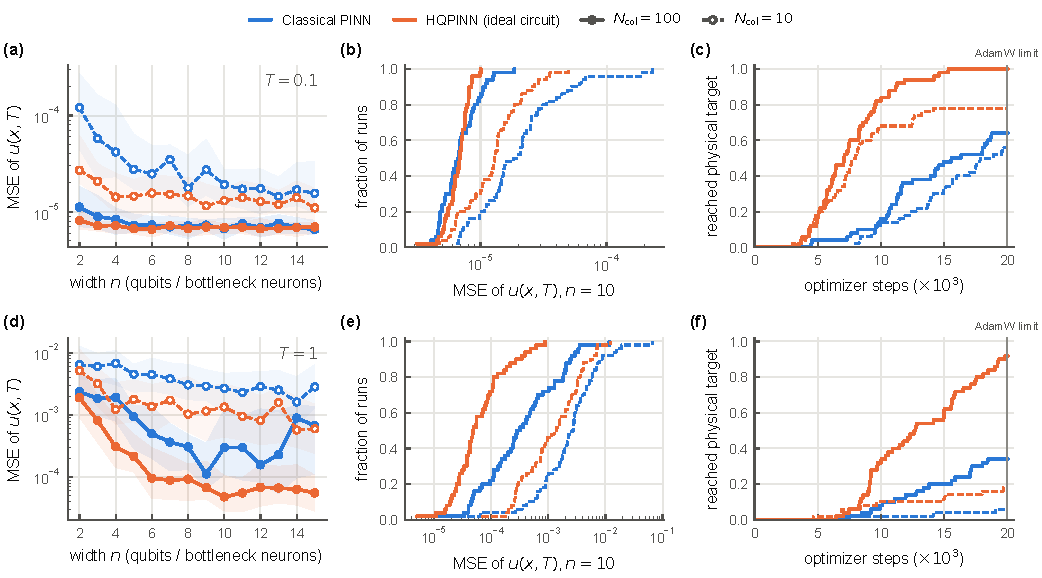
\includegraphics[width=\textwidth]{fig2_simulations.pdf}
  \caption{\justifying Noiseless simulations, classical PINN (blue) and HQPINN with the ideal circuit (orange) trained with the same protocol; 50 seeds per point. Top row, $T=0.1$; bottom row, $T=1$. Solid lines, $\Ncol=100$ collocation points per step; dashed lines with open markers, $\Ncol=10$.
  (a,d) Median MSE of $u(x,T)$ versus the width $n$ of the latent space (number of qubits of the HQPINN, bottleneck width of the classical PINN); bands, interquartile range.
  (b,e) Empirical distribution of the MSE over the 50 seeds for $n=10$.
  (c,f) Fraction of the runs, $n=10$, that have reached the physical stopping target (the residual of the reference solution, Sec.~\ref{sec:methods_sim}) as a function of the number of optimizer steps; the AdamW phase ends at $2\times10^4$ steps.}
  \label{fig:sim}
\end{figure*}

\paragraph{Same protocol, long budget.} Figure~\ref{fig:sim} and Table~\ref{tab:sim} compare the two models over 5600 runs. At $T=0.1$ with $\Ncol=100$ both models reach the same median MSE, $\simeq7\times10^{-6}$ ($\epsilon_{L_2}\simeq0.4\%$) for $n\ge4$ [Fig.~\ref{fig:sim}(a)]; this level is set by the reference solution and is reached by the HQPINN for every $\Ncol\ge30$ (Appendix~\ref{app:extra}). With only $\Ncol=10$ points per step the median MSE of the HQPINN is lower than that of the classical PINN for every width, by a factor between 1.2 and 4.5, and its distribution over seeds is narrower [Fig.~\ref{fig:sim}(b)]. Neither model has failed runs at $T=0.1$ under this protocol (largest MSE $2.2\times10^{-3}$ for the classical PINN and $1.2\times10^{-3}$ for the HQPINN among 1400 runs each). The difference is more pronounced in convergence than in final accuracy: with $\Ncol=100$, 98\% of the HQPINN runs with $n\ge5$ reach the physical target, against 55\% of the classical ones, and for $n=10$ the median run stops after $7.1\times10^3$ steps against $1.6\times10^4$ [Fig.~\ref{fig:sim}(c)].

At $T=1$ the advantage of the HQPINN extends to the final accuracy [Figs.~\ref{fig:sim}(d)--(f)]. Its median MSE is lower for every width and both values of $\Ncol$, by a factor of up to 14 for $\Ncol=100$; for $n=10$ it is $4.8\times10^{-5}$ ($\epsilon_{L_2}=3.3\%$) against $3.0\times10^{-4}$ (8.2\%), and 92\% of the runs reach the target against 34\%. The classical PINN improves non-monotonically with $n$, and its best median ($1.1\times10^{-4}$ at $n=9$, 430 parameters) is above that of the HQPINN for every $n\ge6$ (187 parameters and more) [Fig.~\ref{fig:extra}(c)]. Since the ideal quantum layer is a fixed cosine-product map (Remark~\ref{rem:parity}), these results show that a parameter-free, bounded and periodic middle block conditions the residual minimization better than a trainable bottleneck, in particular for the long horizon; they do not rely on any quantum effect. At the hardware budget [$T=0.1$, 110 epochs, $n=10$, seeds 0--4; Fig.~\ref{fig:ladder}], replacing $\tanh$ by $\sin$ in the classical middle block lowers the median $\epsilon_{L_2}$ from 31.1\% to 20.9\% (7.0--27.2\%) under the learning-rate schedule of the HQPINN (9.1\% for the noiseless HQPINN), and from 11.4\% to 10.6\% (8.7--12.5\%) under the best schedule of the classical model (Sec.~\ref{sec:discussion}): a periodic activation closes part of the gap at a common schedule and has little effect once the schedule is tuned. \TODO{repetir o controle com \texttt{seno=True} no protocolo longo ($T=1$), onde est\'a a vantagem.}

\begin{table}[b]
\caption{\justifying Same-protocol simulations for $n=10$ (50 seeds): median MSE and relative $L_2$ error of $u(x,T)$, fraction of runs reaching the physical target, and median number of optimizer steps. Trainable parameters: 491 (classical), 271 (HQPINN).}
\label{tab:sim}
\setlength{\tabcolsep}{1.5pt}
\footnotesize
\begin{ruledtabular}
\begin{tabular}{llcccc}
$T$, $\Ncol$ & model & MSE & $\epsilon_{L_2}$ & target & steps/$10^3$\\
\colrule
0.1, 10  & class. & $1.9{\times}10^{-5}$ & 0.6\% & 56\% & 18.4\\
         & HQPINN & $1.3{\times}10^{-5}$ & 0.5\% & 78\% & 8.0\\
0.1, 100 & class. & $6.7{\times}10^{-6}$ & 0.4\% & 64\% & 16.0\\
         & HQPINN & $6.9{\times}10^{-6}$ & 0.4\% & 100\% & 7.1\\
1, 10    & class. & $2.7{\times}10^{-3}$ & 24.6\% & 6\% & 20.1\\
         & HQPINN & $1.3{\times}10^{-3}$ & 17.4\% & 18\% & 20.1\\
1, 100   & class. & $3.0{\times}10^{-4}$ & 8.2\% & 34\% & 20.1\\
         & HQPINN & $4.8{\times}10^{-5}$ & 3.3\% & 92\% & 12.7\\
\end{tabular}
\end{ruledtabular}
\end{table}

\paragraph{Hardware budget.} The hardware run is limited to 110 epochs with $\Ncol=10$, two orders of magnitude fewer steps than above, at a large learning rate. At this budget the result depends strongly on the seed [Fig.~\ref{fig:ladder}, simulation rows]: the noiseless HQPINN reaches $\epsilon_{L_2}$ between 3.9\% and 15.1\% (median 9.1\%; 5.5\% for seed 0), and adding 1024-shot noise at the stencil centres does not degrade it (3.8\%--16.2\%, median 5.5\%). The FakeBerlin emulation, with the full noise model of the device, gives 4.1\% for seed 0 and 6.9\%--8.1\% for seeds 1--4. In contrast, the classical PINN trained with the same protocol ends between 4.6\% and 35.9\% (median 24.7\%), and 28\% of its runs end above the no-evolution level. Within the statistics available, neither shot noise nor the noise model of the device is the limiting factor at this budget: the spread is dominated by the short optimization.

\subsection{Real quantum processor}\label{sec:res_qpu}

\begin{figure*}[t]
  \centering
  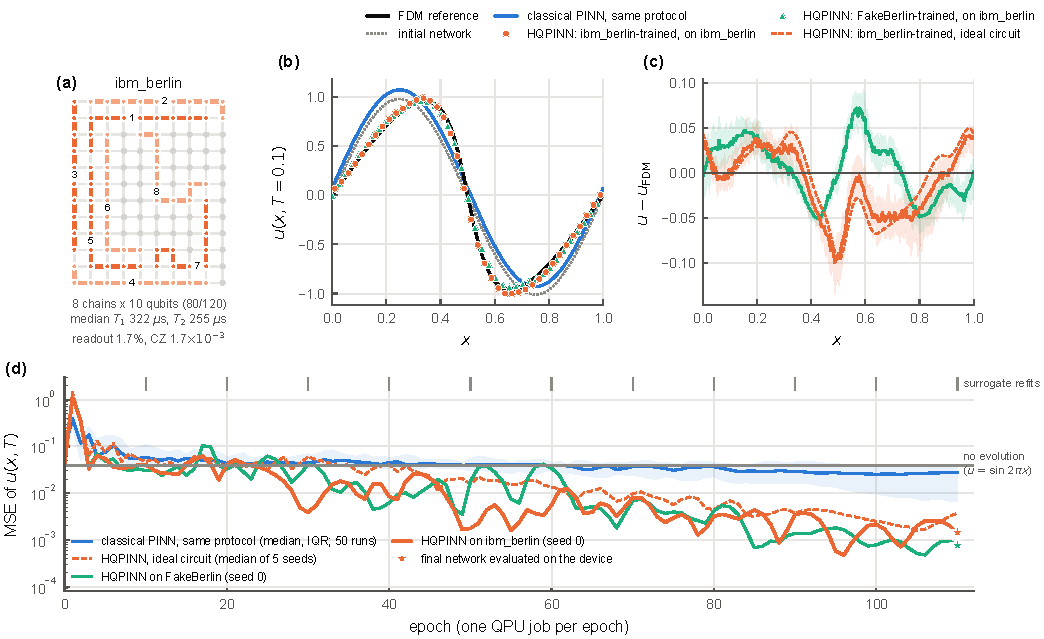
\includegraphics[width=\textwidth]{fig3_hardware.pdf}
  \caption{\justifying Training the HQPINN with \texttt{ibm\_berlin} in the loop ($n=10$, $\Ncol=10$, 110 epochs, seed 0, no error mitigation).
  (a) The 120-qubit square lattice of \texttt{ibm\_berlin} and the 8 disjoint 10-qubit chains on which the circuit ran in parallel (alternating shades and numbers distinguish neighbouring chains); median device figures of the 80 qubits used.
  (b) $u(x,T=0.1)$: FDM reference (black), initial network (dotted), classical PINN trained with the same protocol ($n=10$, blue), HQPINN trained on FakeBerlin and evaluated on \texttt{ibm\_berlin} (triangles), HQPINN trained and evaluated on \texttt{ibm\_berlin} (circles; every fifth point shown).
  (c) Pointwise error of the hardware evaluations; bands, spread (minimum to maximum) of the network output over the 8 chains, each validation point having been measured once on every chain; dashed, the \texttt{ibm\_berlin}-trained weights evaluated with the ideal circuit.
  (d) MSE of $u(x,T)$ versus epoch, from the bit-exact replay of the recorded runs, with the network evaluated through the calibrated surrogate in force at each epoch; stars, final network evaluated on the device (validation job). Blue, median and interquartile range of the classical PINN trained with the same protocol (widths 1--10, seeds 0--4); dashed orange, median of the noiseless HQPINN (seeds 0--4). Ticks at the top mark the surrogate refits; the learning rate decreases from 0.1 to 0.01 in steps every 10 epochs.}
  \label{fig:hardware}
\end{figure*}

\paragraph{Training on the device.} Figure~\ref{fig:hardware} shows the HQPINN trained with \texttt{ibm\_berlin} in the loop. The network, initialized at $\epsilon_{L_2}=29.4\%$, ends at $\mathrm{MSE}=1.45\times10^{-3}$ ($\epsilon_{L_2}=5.7\%$) when evaluated with the circuit running on the device, a 27-fold reduction of the MSE, and follows the steep front at $x\simeq0.5$ [Fig.~\ref{fig:hardware}(b)]. The classical PINN trained with the same protocol and the same seed remains close to the initial profile, with the peak and the trough displaced. The replayed learning curve [Fig.~\ref{fig:hardware}(d)] shows a transient of a few epochs at the initial learning rate, falls below $10^{-2}$ at epoch 29, and has a median MSE of $1.9\times10^{-3}$ over the last 10 epochs, against $2.7\times10^{-2}$ for the classical control. After epoch 30 the \texttt{ibm\_berlin} and FakeBerlin curves lie at or below the median curve of the noiseless HQPINN in 88\% and 85\% of the epochs, respectively. Only one of the 50 classical runs ends below the MSE of the hardware run. The pointwise error [Fig.~\ref{fig:hardware}(c)] is largest at the front ($|u-u_{\rm FDM}|\le0.1$); the spread between the 8 chains is small compared with this systematic error, and the same weights evaluated with the ideal circuit give $\epsilon_{L_2}=6.0\%$, so the trained network is not tied to the specific noise of the chip.

\begin{figure}[t]
  \centering
  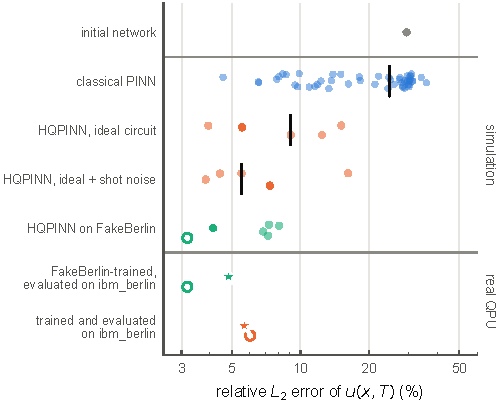
\includegraphics[width=\linewidth]{fig4_noise_ladder.pdf}
  \caption{\justifying Relative $L_2$ error of $u(x,T=0.1)$ at the hardware budget (110 epochs, $\Ncol=10$), from noiseless simulation to the real QPU. Simulation: classical PINN (widths 1--10, seeds 0--4), HQPINN with the ideal circuit and with 1024-shot noise (seeds 0--4), and HQPINN on FakeBerlin (seed 0 on the chains of the real run; small markers, seeds 1--4 of an earlier FakeBerlin batch). Real QPU: the FakeBerlin-trained network evaluated on \texttt{ibm\_berlin}, and the network trained and evaluated on \texttt{ibm\_berlin}. Large markers, seed 0 (the seed of the hardware runs); open markers, the same weights evaluated with the ideal circuit; vertical ticks, medians.}
  \label{fig:ladder}
\end{figure}

\paragraph{Transfer between emulator and device.} The network trained on FakeBerlin and evaluated on \texttt{ibm\_berlin} gives $\epsilon_{L_2}=4.8\%$, against 4.1\% on the emulator (Fig.~\ref{fig:ladder} and Table~\ref{tab:hw}): the noise model transfers to the real device with a small loss. Training on the real device (5.7\%) and training on the emulator (4.8\% on the device) lead to comparable results; with one seed each, both lie within the seed-to-seed spread of the noiseless model, so neither strategy can be declared superior. The real run lies above the same seed on the FakeBerlin batch (4.2\%) but within the range of the five FakeBerlin seeds, which is compatible with the effects of drift and chain-to-chain variation that the emulator does not model (Sec.~\ref{sec:res_device}).

\begin{table}[b]
\caption{\justifying HQPINN at the hardware budget ($n=10$, $\Ncol=10$, 110 epochs, $T=0.1$): MSE and relative $L_2$ error of $u(x,T)$. Rows marked $^{a}$ give the median over seeds 0--4 (ranges of $\epsilon_{L_2}$: ideal circuit 3.9--15.1\%, with shot noise 3.8--16.2\%) or, for the classical control, over widths 1--10 and seeds 0--4 (4.6--35.9\%); all other rows are seed 0.}
\label{tab:hw}
\setlength{\tabcolsep}{2.5pt}
\footnotesize
\begin{ruledtabular}
\begin{tabular}{llcc}
trained on & evaluated on & MSE & $\epsilon_{L_2}$\\
\colrule
\multicolumn{4}{l}{\emph{Simulation}}\\
ideal circuit$^{a}$ & ideal circuit & $3.7\times10^{-3}$ & 9.1\%\\
ideal + shot noise$^{a}$ & ideal circuit & $1.4\times10^{-3}$ & 5.5\%\\
FakeBerlin & FakeBerlin & $7.7\times10^{-4}$ & 4.1\%\\
FakeBerlin & ideal circuit & $4.6\times10^{-4}$ & 3.2\%\\
\multicolumn{4}{l}{\emph{Real QPU}}\\
FakeBerlin & \texttt{ibm\_berlin} & $1.06\times10^{-3}$ & 4.8\%\\
\texttt{ibm\_berlin} & \texttt{ibm\_berlin} & $1.45\times10^{-3}$ & 5.7\%\\
\texttt{ibm\_berlin} & surrogate $\hat f$ & $1.35\times10^{-3}$ & 5.5\%\\
\texttt{ibm\_berlin} & ideal circuit & $1.64\times10^{-3}$ & 6.0\%\\
\colrule
\multicolumn{2}{l}{initial network} & $3.90\times10^{-2}$ & 29.4\%\\
\multicolumn{2}{l}{classical PINN, same protocol$^{a}$} & $2.8\times10^{-2}$ & 24.7\%\\
\end{tabular}
\end{ruledtabular}
\end{table}

\subsection{Fidelity of the device model}\label{sec:res_device}
Figure~\ref{fig:device} quantifies how well the calibrated surrogate describes the device. On FakeBerlin the calibration residual is at the shot-noise level (RMS 0.029 against 0.028 expected from 1024 shots), the contrast of the ideal term $\prod_{j\in\mathcal S_q}\cos\theta_j$ is 0.93--0.96 for all outputs, and the misfit of every chain is at the shot-noise floor: the emulated device is fully described by Eq.~\eqref{eq:trigpoly} with chip-averaged coefficients. On \texttt{ibm\_berlin} the contrast is lower and more heterogeneous (0.86--0.96), the residual distribution has heavier tails (RMS 0.044), and one chain has twice the median misfit [Figs.~\ref{fig:device}(a)--(c)]. During training the RMS of the correction $\Delta=\hat{\bm y}^{\,\rm QPU}-\hat f$ at the stencil centres stays at the shot-noise level on FakeBerlin (mean 0.030) and at 0.031--0.076 (mean 0.045) on \texttt{ibm\_berlin}, with averages over every 10 epochs between 0.042 and 0.050 [Fig.~\ref{fig:device}(d)]: the device did not drift away from the model during the 29~min of training. At validation, where every point is averaged over the 8 chains, the RMS drops to 0.013, close to the floor $1/(32\sqrt8)=0.011$. An excess that averages out over chains is chain-specific rather than common to the chip, which identifies chain-to-chain variation as the main limitation of a chip-averaged surrogate; chain-resolved coefficients would remove it at the cost of $B$ times more calibration samples.

\begin{figure*}[t]
  \centering
  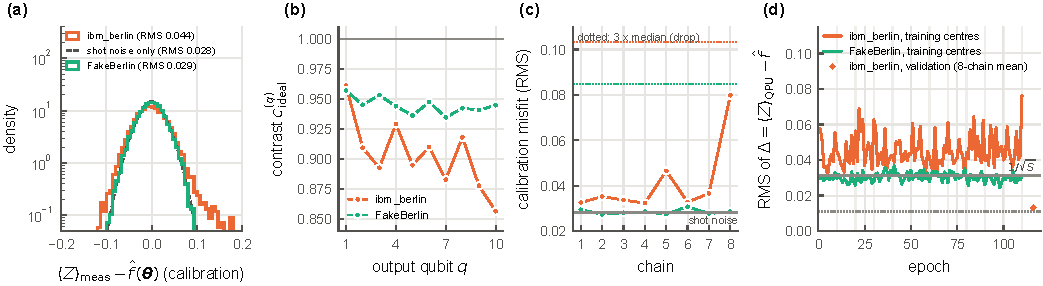
\includegraphics[width=\textwidth]{fig5_device_model.pdf}
  \caption{\justifying Calibrated surrogate versus device, \texttt{ibm\_berlin} (orange) and FakeBerlin (aqua).
  (a) Distribution of the residual of the calibration fit, $\langle Z\rangle_{\rm meas}-\hat f(\bm\theta)$, over 1024 random angle sets and 10 outputs; dashed, the distribution expected from 1024-shot noise alone.
  (b) Contrast, the fitted coefficient of the ideal term $\prod_{j\in\mathcal S_q}\cos\theta_j$ of each output (1 for a noiseless device).
  (c) Misfit of each chain to the chip-averaged surrogate; dotted, the screening threshold ($3\times$ median); grey, shot-noise level.
  (d) RMS of the measured correction $\Delta$ at the stencil centres per training epoch (surrogate refitted every 10 epochs, light vertical lines) and at validation (diamond, 8-chain average); horizontal lines, the shot-noise levels $1/\sqrt S$ and $1/\sqrt{8S}$.}
  \label{fig:device}
\end{figure*}

% =====================================================================
\section{Discussion}\label{sec:discussion}
% =====================================================================
\TODO{Rascunho -- revisar.} Three points frame the results. First, the comparison in simulation is between two classical computations: the noiseless quantum layer is a fixed cosine-product map (Remark~\ref{rem:parity}), and its better conditioning of the residual minimization---higher success rate, half the optimizer steps, about half the parameters, and an up to 14-fold (6-fold for $n=10$) lower error at the long horizon---is an architectural effect. The quantum processor enters as the physical device that implements this map, and the question addressed by the hardware experiment is whether such a model can be \emph{trained} through a noisy device. Second, the answer is positive at the budget tested: with one job per epoch, without error mitigation, on 80 qubits, the network reaches an accuracy indistinguishable from that of the noiseless model trained with the same protocol. Proposition~\ref{prop:trig} is what makes this possible, since noise changes the coefficients of the layer but not its functional form, so a calibrated model of the device provides both the gradient and a noise-free interpolation across the finite-difference stencil. Third, the straight-through construction is generic: it applies to any circuit whose light cones are small enough for the $3^{|\mathcal C_q|}$ coefficients of Eq.~\eqref{eq:trigpoly} to be calibrated, which bounds the entangling depth to a few brickwork layers, and it is compatible with error mitigation schemes that are affine in the measured data (e.g., readout mitigation~\cite{vandenberg2022model}, Pauli twirling, linear zero-noise extrapolation~\cite{temme2017error}).

\emph{Limitations.} The hardware results rest on one seed per training strategy, and that seed was the best of five on the emulator. The classical control at the hardware budget uses the learning-rate schedule selected for the HQPINN; a schedule tuned for the classical model would narrow the gap at that budget: for $n=10$, the best of ten schedules (the step decay of the HQPINN rescaled to $\eta_0$, or a cosine decay from $\eta_0$ to $\eta_0/10$, with $\eta_0\in\{1,3,10,30,100\}\times10^{-3}$), selected on the test error itself, is a cosine decay from $\eta_0=0.03$; it lowers the median $\epsilon_{L_2}$ from 31.1\% to 11.4\% (6.2--19.5\%, MSE $5.8\times10^{-3}$), against 9.1\% (3.9--15.1\%, $3.7\times10^{-3}$) for the noiseless HQPINN and 5.7\% for the run on \texttt{ibm\_berlin}. For $n=3$ the schedule of the HQPINN is already the best (13.7\%). The long-budget comparison uses a common protocol, not separately optimized hyperparameters. Finally, the stopping target and the error metric rely on a first-order finite-difference reference whose own error sets the $7\times10^{-6}$ floor.

% =====================================================================
\section{Conclusions}\label{sec:conclusions}
% =====================================================================
\TODO{Conclus\~oes -- a escrever.}
% Outlook items: inverse problem (identification of nu, previous draft); chain-resolved surrogates;
% error mitigation; deeper entangling layers (|C_q| <= 4D); larger n and harder PDEs; seismic inversion.

\begin{acknowledgments}
\TODO{Agradecimentos; acesso ao IBM Quantum (inst\^ancia PDE\_Europe); financiamento.}
\end{acknowledgments}

% =====================================================================
\begin{appendices}
% =====================================================================

\section{Reference solution and error metrics}\label{app:reference}
The reference $u_{\rm FDM}$ is obtained with an explicit scheme on $N_x=512$ periodic grid points ($\Delta x=1/512$) with time step $\Delta t=10^{-4}$: first-order upwind differences for the advection term, $u\,\partial_xu\to u_j(u_j-u_{j-1})/\Delta x$ for $u_j\ge0$ and $u_j(u_{j+1}-u_j)/\Delta x$ otherwise, and second-order central differences for the diffusion term. The time step satisfies the advective and diffusive stability limits ($\Delta t\max|u|/\Delta x\simeq0.05$, $\nu\Delta t/\Delta x^2\simeq0.26$). Evaluation points that do not coincide with the grid are obtained by periodic linear interpolation at $t=T$.

\emph{FDM floor.} The stopping target of the simulations is the residual of the reference itself, $\mathcal L_{\rm FDM}=\frac{1}{N}\sum_k r_k[u_{\rm FDM}]^2$, evaluated with the same stencil $(h,\tau)$ on the same validation points, with $u_{\rm FDM}$ interpolated bilinearly (periodic in $x$, linear in $t$). Because the upwind scheme is only first-order accurate, $\mathcal L_{\rm FDM}>0$; a network whose residual is below it would be fitting the error of the reference. The corresponding floor of the MSE against the reference is $\simeq7\times10^{-6}$ at $T=0.1$.

\emph{Metrics.} $\mathrm{MSE}=\frac1P\sum_p[u(x_p,T)-u_{\rm FDM}(x_p,T)]^2$, $\mathrm{MAE}$ analogously, and $\epsilon_{L_2}=\|u-u_{\rm FDM}\|_2/\|u_{\rm FDM}\|_2$, on $P=200$ equispaced points $x_p\in[0,1]$. At $T=0.1$, $\langle u_{\rm FDM}^2\rangle=0.453$, so $\epsilon_{L_2}=\sqrt{\mathrm{MSE}/0.453}$.

\section{Proof of Proposition~\ref{prop:trig} and light-cone structure}\label{app:trig}
\emph{Trigonometric structure.} For a single rotation,
\begin{align}
  R_Y(\theta)\,\rho\,R_Y^\dagger(\theta)={}&\tfrac12(\rho+Y\rho Y)+\tfrac12\cos\theta\,(\rho-Y\rho Y)\nonumber\\
  &-\tfrac{i}{2}\sin\theta\,[Y,\rho],
  \label{eq:ry_channel}
\end{align}
so the map $\rho\mapsto R_Y(\theta)\rho R_Y^\dagger(\theta)$ is an affine combination of $\{1,\cos\theta,\sin\theta\}$ with $\theta$-independent superoperators. All other operations---CNOTs, noise channels, readout confusion matrices and the trace with $Z_q$---are linear and $\theta$-independent. Since each angle appears in exactly one gate, $y_q$ is a sum of products in which every $\theta_j$ contributes exactly one factor in $\{1,\cos\theta_j,\sin\theta_j\}$, which is Eq.~\eqref{eq:trigpoly}.

\emph{Light cone.} In the Heisenberg picture $y_q=\operatorname{Tr}[\rho_0\,\mathcal E^\dagger_{\bm\theta}(Z_q)]$. The adjoint of a trace-preserving channel is unital, so every gate (and every gate-local noise channel) whose support does not intersect the current support of the evolved operator leaves it unchanged. The support grows only through gates that touch it; the set of qubits reached is $\mathcal C_q$, and rotations outside $\mathcal C_q$ drop out. Going backwards through one brickwork layer, the second sublayer adds at most the partner of $q$ and the first sublayer at most one qubit on each side, so $|\mathcal C_q|\le4$; for $D$ layers, $|\mathcal C_q|\le\min(n,4D)$. For $n=10$ the cones are $\{1,2\}$, $\{1,\dots,4\}$ (twice), $\{3,\dots,6\}$ (twice), $\{5,\dots,8\}$ (twice), $\{7,\dots,10\}$ (twice) and $\{9,10\}$. Crosstalk or non-local noise invalidates this bound and enlarges the effective cone.

\emph{Noiseless case (Remark~\ref{rem:parity}).} CNOT conjugation maps $Z_c\mapsto Z_c$ and $Z_t\mapsto Z_cZ_t$, so $Z_q$ evolves into the string $Z_{\mathcal S_q}$ whose support is the $q$th row of the GF(2) matrix $M$ of the network. On $\bigotimes_jR_Y(\theta_j)|0\rangle$, $\langle Z_j\rangle=\cos\theta_j$ and the state is a product, which gives Eq.~\eqref{eq:parity}. For one brickwork layer on $n=10$ qubits the supports are $\mathcal S_1=\{1\}$, $\mathcal S_2=\{1,2\}$, $\mathcal S_{q}=\{q-2,q-1,q\}$ for odd $q\ge3$, $\mathcal S_q=\{q-1,q\}$ for even $q\ge4$, so that, e.g., $y_3=\cos\theta_1\cos\theta_2\cos\theta_3$ and $y_{10}=\cos\theta_9\cos\theta_{10}$; hence $|\mathcal S_q|\le3$ and $\mathcal S_q\subsetneq\mathcal C_q$ for most outputs. If the $\theta_j$ are independent and uniform on a period, $\mathbb E[\cos^2\theta_j]=1/2$, hence $\operatorname{Var}[y_q]=2^{-|\mathcal S_q|}$ and $\mathbb E[(\partial_{\theta_j}y_q)^2]=2^{-|\mathcal S_q|}$.

\emph{Conditioning of the calibration.} With $\theta_j\sim\mathcal U(-\pi,\pi)$ i.i.d., the features $\prod_{j\in\mathcal C_q}g_{\alpha_j}(\theta_j)$ are orthogonal, with $\mathbb E[g_0^2]=1$ and $\mathbb E[g_c^2]=\mathbb E[g_s^2]=1/2$. The Gram matrix of the least-squares problem is therefore diagonal in expectation, with condition number $2^{|\mathcal C_q|}\le16$, and the standard error of a coefficient with $k$ non-constant factors is $\simeq\sigma\,2^{k/2}/\sqrt{N_{\rm cal}}$. With $N_{\rm cal}=1024$ samples and $\sigma\simeq1/32$, the highest-order coefficients ($k=4$) are determined to $\simeq4\times10^{-3}$, well below the shot noise of a single measurement.

\section{Training algorithms}\label{app:training}

\begin{algorithm}{Simulation training (classical PINN and ideal HQPINN), long budget.}\label{alg:sim}
\item \textbf{input:} width $n$, $\Ncol$, horizon $T$, seed $s$; stencil $(h,\tau)$; $K_{\rm A}=2\times10^4$, $K_{\rm B}=10^3$
\item set seed $s$; initialize $\Theta$; draw a fixed validation set $\mathcal V$ of $\Ncol$ points (seed $10^6+s$)
\item $\mathcal L_{\rm FDM}\gets$ residual of the reference on $\mathcal V$ (Appendix~\ref{app:reference})
\item \textbf{for} $k=1,\dots,K_{\rm A}$: draw $\Ncol$ points; build the $5\Ncol$ stencil nodes; $\Theta\gets$ AdamW$(\nabla_\Theta\mathcal L)$; evaluate $\mathcal L(\mathcal V)$; keep the best snapshot; \textbf{stop} if $\mathcal L(\mathcal V)\le\mathcal L_{\rm FDM}$
\item restore the best snapshot; \textbf{for} $k=1,\dots,K_{\rm B}$: one L-BFGS iteration on the last batch; evaluate $\mathcal L(\mathcal V)$; \textbf{stop} at the target or after 50 iterations without improvement
\item \textbf{return} the best snapshot
\end{algorithm}

\begin{algorithm}{HQPINN training with the quantum processor in the loop.}\label{alg:hil}
\item \textbf{input:} chains $\{\mathcal Q_b\}_{b=1}^{B}$, shots $S$, epochs $K$, $\Ncol$, refit period $K_{\rm fit}$, schedule $\eta_k$
\item \emph{calibration job}: $\lceil1024/B\rceil$ random angle sets on all chains $\to(\bm\theta,\hat{\bm y})$; screen chains; fit $\hat f$ [Eq.~\eqref{eq:trigpoly}]
\item set seed; initialize $\Theta=(\bm\phi,\bm\psi)$
\item \textbf{for} $k=1,\dots,K$:
\item \quad draw $\Ncol$ centres; stencil nodes $\mathcal S$; $\bm\theta\gets\mathcal N_{\rm pre}(\bm\xi(\mathcal S))$
\item \quad \emph{job $k$}: measure $\hat{\bm y}_c$ at the centres; centre $p$ runs on chain $(p+k)\bmod B$
\item \quad $\tilde{\bm y}\gets\hat f(\bm\theta)+\sg[\hat{\bm y}_c-\hat f(\bm\theta_c)]$ on all nodes [Eq.~\eqref{eq:ste}]
\item \quad $u\gets$ Eq.~\eqref{eq:composition}; $\mathcal L\gets$ Eq.~\eqref{eq:loss}; backward through $\hat f$; clip $\|\nabla\|\le1$; AdamW step with $\eta_k$
\item \quad \textbf{if} $k\bmod K_{\rm fit}=0$: refit $\hat f$ with the calibration and all measurements so far
\item \emph{validation job}: $u(x,T)$ on 200 points, each measured on every chain and averaged
\end{algorithm}

Both models are trained with Algorithm~\ref{alg:sim} in the long-budget simulations; the HQPINN on FakeBerlin and on \texttt{ibm\_berlin} with Algorithm~\ref{alg:hil}; the classical control and the hardware-budget simulations follow the loop of Algorithm~\ref{alg:hil} with the device replaced by the classical middle block or by the ideal layer (with or without sampled shot noise). The learning rate is set at every epoch, $\eta_k=\max\{0.1-0.01\lfloor(k-1)/10\rfloor,\,0.01\}$, and the AdamW state is kept across epochs.

\section{Straight-through estimator and finite differences}\label{app:ste}
\emph{Stencil formulas and truncation.} On the cross stencil,
\begin{align}
  \partial_tu&\approx\frac{u(x,t+\tau)-u(x,t-\tau)}{2\tau},\qquad \partial_xu\approx\frac{u_{+}-u_{-}}{2h},\nonumber\\
  \partial_x^2u&\approx\frac{u_{+}-2u_0+u_{-}}{h^2},\qquad u_\pm=u(x\pm h,t),
\end{align}
with truncation errors $\tfrac{\tau^2}{6}\partial_t^3u$, $\tfrac{h^2}{6}\partial_x^3u$ and $\tfrac{h^2}{12}\partial_x^4u$; for $h=1/512$ and $\tau=10^{-3}$ these are negligible against the other errors of the method.

\emph{Noise amplification.} If each node carried independent noise of standard deviation $\sigma_u$ (shot noise $\le1/\sqrt S$ in $y_q$ propagated through $\mathcal N_{\rm post}$), the derivative estimates would have
\begin{equation}
  \operatorname{std}[\partial_xu]=\frac{\sigma_u}{\sqrt2\,h},\qquad \operatorname{std}[\partial_x^2u]=\frac{\sqrt6\,\sigma_u}{h^2}.
\end{equation}
With $h=1/512$ and $\sigma_u\sim10^{-2}$, $\operatorname{std}[\partial_x^2u]\sim6\times10^3$, three orders of magnitude above $|\partial_x^2u|$ away from the front. Enlarging $h$ to make this tolerable would introduce a truncation bias in the residual.

\emph{Shared offset.} Eq.~\eqref{eq:ste} assigns the same correction $\Delta_c=\hat{\bm y}^{\,\rm QPU}(\bm\theta_c)-\hat f(\bm\theta_c)$ to the five nodes of the stencil. Writing $\tilde{\bm y}_\pm=\hat f(\bm\theta_\pm)+\Delta_c$ and expanding $\mathcal N_{\rm post}$,
\begin{equation}
  u_+-u_-=\tfrac{t}{T}J(\hat f_c+\Delta_c)\,\big[\hat f(\bm\theta_+)-\hat f(\bm\theta_-)\big]+\mathcal O(h^3),
\end{equation}
where $J$ is the Jacobian of $\mathcal N_{\rm post}$. The noise enters only through the evaluation point of $J$, so it perturbs the derivatives by a relative amount $\mathcal O(\|J'\|\,\|\Delta_c\|)$ instead of $\mathcal O(\sigma_u/h^2)$. The measured value enters the factor $u$ of $u\,\partial_xu$ directly.

\emph{Gradient bias.} The backward pass uses $\partial\hat f/\partial\bm\theta$ instead of the (inaccessible) derivative of the device response. By Proposition~\ref{prop:trig} both are derivatives of trigonometric polynomials of the same form, so the bias is the derivative of the coefficient error and of the unmodelled part of the response. Parameter-shift rules would give an unbiased but noisy estimate of the same quantity from $2n$ additional circuits per point~\cite{schuld2019evaluating,wierichs2022general}; the surrogate replaces them by one regression over all measurements, in the spirit of model-based optimizers for variational algorithms~\cite{sung2020using,nakanishi2020sequential,ostaszewski2021structure}.

\begin{table}[b]
\caption{\justifying Circuit evaluations per epoch for the gradient of the residual loss ($\Ncol=10$, five stencil nodes per point, $n=10$ angles per node). Parameter shift, SPSA and finite differences require measuring every stencil node, so the shot noise of $\partial_x^2u$ is amplified by $\sim h^{-2}$.}
\label{tab:cost}
\setlength{\tabcolsep}{2pt}
\footnotesize
\begin{ruledtabular}
\begin{tabular}{lll}
method & circuits/epoch & noise in $\partial_x^2u$\\
\colrule
surrogate + STE (this work) & 10 (1 job) & not amplified\\
parameter shift & $\simeq1050$ & $\times\,h^{-2}$\\
SPSA & $\simeq100$ & $\times\,h^{-2}$\\
finite differences in $\bm\theta$ & $\simeq1050$ & $\times\,h^{-2}$\\
\end{tabular}
\end{ruledtabular}
\end{table}

\section{Implementation of the hardware loop}\label{app:hil_impl}
\paragraph{Chains.} All disjoint chains of $n$ physically coupled qubits are searched on the coupling map with a randomized greedy depth-first search that starts from the qubits with fewest free neighbours (100 trials; the largest set is kept). Each chain is scored by the sum of its readout and $\sqrt X$ errors and of the CZ errors of its links, and chains with a score above $0.05\,n$ are discarded; on \texttt{ibm\_berlin} 8 of 12 candidate chains were kept (rejected scores 0.51, 0.57, 1.27, 3.83). The circuit is laid out on all kept chains in a single packed circuit, so that one parameter set yields one sample per chain; transpilation with an initial layout on the chains produced no SWAP (72 CZ, depth 12).

\paragraph{Calibration and screening.} The calibration job evaluates 128 random angle sets on the 8 chains (1024 samples per output). Since the chains are physically different, each chain is also screened: its RMS misfit to the chip-averaged surrogate is computed, and chains above three times the median are discarded. On \texttt{ibm\_berlin} the misfits were 0.032--0.080 and all chains were kept. The surrogate is a single set of coefficients for the whole chip; the per-output fit RMS was 0.025--0.095 (mean 0.039, shot noise 0.031) and the RMS difference between the device and the ideal formula 0.064 (FakeBerlin: 0.028 and 0.039).

\paragraph{Training jobs.} The 10 stencil centres of each epoch fill 2 parameter sets on the 8 chains; centre $p$ runs on chain $(p+k)\bmod8$ at epoch $k$, which rotates the points over the chains and prevents a systematic assignment of points to poor chains. The surrogate is refitted every 10 epochs with the calibration data and all training measurements (1124 to 2124 samples). An epoch took 16~s on average, dominated by job latency inside the session; on the emulator, 3.5~s.

\paragraph{Validation.} The validation job evaluates the 200 points at $t=T$ with 8 replicas, one on every chain, and averages $\hat{\bm y}$ over the replicas before the post-network, so the average matches the chip-averaged surrogate. Three evaluations of the same weights are reported: with the circuit on the device, with the surrogate, and with the ideal formula.

\paragraph{Offline replay.} The run log contains the initial weights, the calibration data and, for every epoch, the collocation points, the angles sent to the device and the measured $\hat{\bm y}$. Replaying Algorithm~\ref{alg:hil} with the recorded measurements in place of the device reproduces the trained weights, the training losses and the angles of every epoch exactly (maximum difference zero, for both \texttt{ibm\_berlin} and FakeBerlin), which we use to evaluate the network after each epoch [Fig.~\ref{fig:hardware}(d)] without additional quantum resources.

\begin{table}[b]
\caption{\justifying \texttt{ibm\_berlin} on 8 October 2026: the 80 qubits and 72 couplers used (median and range).}
\label{tab:device}
\setlength{\tabcolsep}{4pt}
\footnotesize
\begin{ruledtabular}
\begin{tabular}{lcc}
quantity & median & range\\
\colrule
$T_1$ & 322~$\mu$s & 110--528~$\mu$s\\
$T_2$ & 255~$\mu$s & 34--510~$\mu$s\\
readout error & 1.7\% & 0.5--6.3\%\\
$\sqrt X$ error & $1.7\times10^{-4}$ & $(0.7$--$9.9)\times10^{-4}$\\
CZ error & $1.7\times10^{-3}$ & $(0.6$--$14)\times10^{-3}$\\
\colrule
qubits used / total & \multicolumn{2}{c}{80 / 120 (8 chains $\times$ 10)}\\
packed circuit & \multicolumn{2}{c}{depth 12, 72 CZ, no SWAP}\\
jobs / shots / time & \multicolumn{2}{c}{112 / $5.6\times10^5$ / 54 min}\\
\end{tabular}
\end{ruledtabular}
\end{table}

\section{Architectures and hyperparameters}\label{app:hyper}

\begin{table}[h]
\caption{\justifying Network architectures (all hidden layers $\tanh$, linear outputs).}
\label{tab:arch}
\setlength{\tabcolsep}{2pt}
\footnotesize
\begin{ruledtabular}
\begin{tabular}{lcc}
 & HQPINN & classical PINN\\
\colrule
features & $\bm\xi$, Eq.~\eqref{eq:composition} & same\\
$\mathcal N_{\rm pre}$ & $3\to10\to n$ & $3\to10\to n$\\
middle block & $R_Y$, $W_{\rm brick}$, $\langle Z_q\rangle$ & $n\to m\to n$\\
$\mathcal N_{\rm post}$ & $n\to10\to1$ & $n\to10\to1$\\
param., middle & 0 & $2nm+m+n$\\
param., total & $21n+61$ & $2n^2+23n+61$ $(m{=}n)$\\
 & & $42n+71$ $(m{=}10)$\\
$n=10$ & 271 & 491\\
\end{tabular}
\end{ruledtabular}
\end{table}

\begin{table}[h]
\caption{\justifying Training hyperparameters. Long budget: same-protocol simulations (Fig.~\ref{fig:sim}). Hardware budget: FakeBerlin, \texttt{ibm\_berlin}, classical control and hardware-budget simulations (Figs.~\ref{fig:hardware}--\ref{fig:device}).}
\label{tab:hyper}
\setlength{\tabcolsep}{2pt}
\footnotesize
\begin{ruledtabular}
\begin{tabular}{lcc}
 & long budget & hardware budget\\
\colrule
$\Ncol$ per step & 10, 100 & 10\\
stencil $(h,\tau)$ & $(1/512,10^{-3})$ & same\\
optimizer & AdamW, L-BFGS & AdamW\\
steps & $\le2{\times}10^4+10^3$ & 110\\
learning rate & $10^{-3}$, plateau $\times\frac12$ & 0.1 to 0.01\\
weight decay; clip & $10^{-6}$; 1 & $10^{-6}$; 1\\
L-BFGS & lr 0.5, hist.\ 50 & --\\
stopping & FDM floor & fixed budget\\
shots $S$ & -- & 1024\\
calibration & -- & 1024 samples\\
refit $K_{\rm fit}$ & -- & 10 epochs\\
seeds & 0--49 & 0 (QPU), 0--4\\
\end{tabular}
\end{ruledtabular}
\end{table}

\section{Additional simulation results}\label{app:extra}

\begin{figure*}[t]
  \centering
  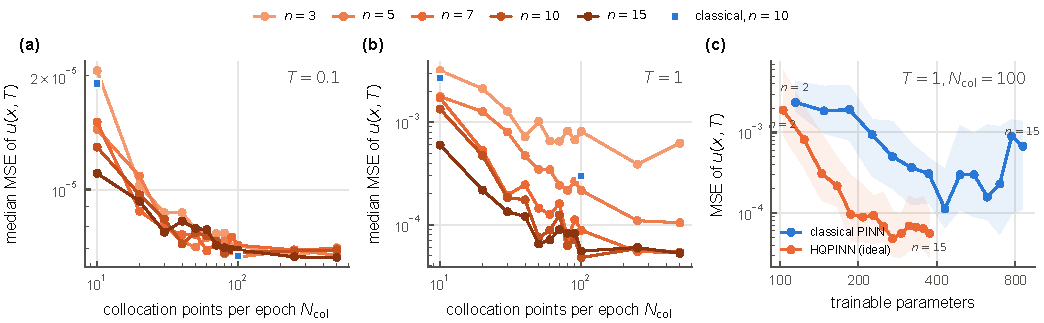
\includegraphics[width=\textwidth]{figS1_exact_ncol.pdf}
  \caption{\justifying (a,b) Median MSE of the noiseless HQPINN versus the number of collocation points per step for $n=3,5,7,10,15$ qubits (light to dark), at $T=0.1$ and $T=1$ (50 seeds, long-budget protocol); squares, classical PINN with $n=10$. (c) Median MSE versus the number of trainable parameters at $T=1$, $\Ncol=100$, for widths $n=2,\dots,15$; bands, interquartile range.}
  \label{fig:extra}
\end{figure*}

At $T=0.1$ the HQPINN reaches the FDM-limited floor for every $\Ncol\ge30$, independently of the number of qubits [Fig.~\ref{fig:extra}(a)]. At $T=1$ the error keeps decreasing up to $\Ncol\simeq100$ and saturates at $\simeq5\times10^{-5}$ for $n\ge7$ [Fig.~\ref{fig:extra}(b)]; the three-qubit model saturates an order of magnitude higher, which identifies the width of the latent space, and not the collocation budget, as the limiting factor at the long horizon.

\section{Data and code availability}\label{app:data}
\TODO{Reposit\'orio/Zenodo.} Every figure is generated by the scripts in \texttt{manuscript/scripts/} from the data in \texttt{data/}: \texttt{fig2\_simulations.py} (same-protocol sweep), \texttt{fig3\_hardware.py}, \texttt{fig4\_noise\_ladder.py} and \texttt{fig5\_device\_model.py} (hardware and emulator runs, classical control), \texttt{figS1\_exact\_ncol.py}; \texttt{replay\_training.py} and \texttt{simulate\_same\_budget.py} produce the replayed learning curves and the hardware-budget simulations without any quantum job. The IBM job identifiers of all 113 hardware jobs are recorded in the run logs.

\end{appendices}

\bibliography{references}

\end{document}
